\section{High Granularity Calorimeter} \label{section:simulations_hgc}

\begin{figure}[hbp]
    \centering
    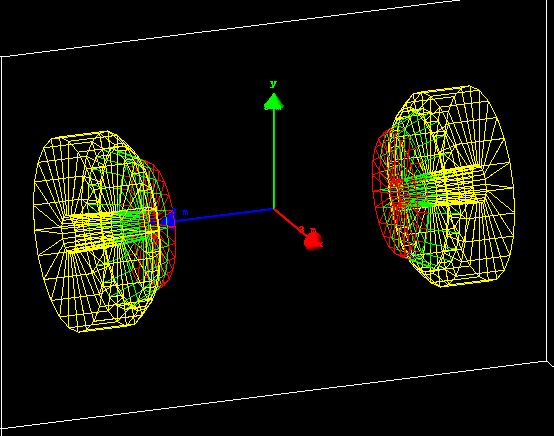
\includegraphics[width=0.9\textwidth]{figures/ch_simulations/hgc/detetor_3d/HGC_70_20.png}
    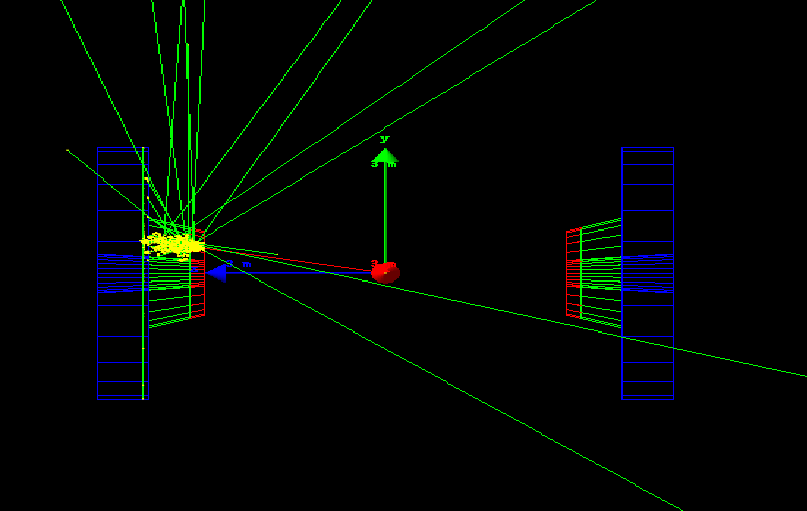
\includegraphics[width=0.9\textwidth]{figures/ch_simulations/hgc/detetor_3d/HGCal_1Event_NoSides.png}
    \caption{Full CMS Scale High Granularity Calorimeter (Top). Example of a Particle Gun response (Bottom)}
    \label{fig:simulations_hgcexamples}
 \end{figure}

\subsection{Physical Layout}
High Granularity Calorimeter consists of three parts: Electromagnetic (EM)Calorimeter, Front Hadronic (FH) and Backing (BH) Calorimeters. Both EM and FH have similar design principles: alternating layers of absorber (we use tungsten) and active materials (Silicon) mixed in together with a layer of electronics readout. Full geometry specification for the EM part can be summaried as follows:
\begin{itemize}
    \item 25 Radiation Length ($X_{0}$) Device
    \item In total 30 layers, where each layer is (absorber (W), active (Si), readout (G10/PCB)).
    \item First 10 layers have $0.5 X_{0}$ per layer
    \item Second 10 layers have $0.8 X_{0}$ per layer
    \item Third 10 layers have $1.2 X_{0}$ per layer
    \item XY-plane is subdivided into pads, with an area of each channel of 0.9 $cm^2$ for the first 20 layers and 1.8 $cm^2$ for the last 10.
\end{itemize}
Full specification for the FH part can be summarized as follows:
\begin{itemize}
    \item 4 Interaction length ($\lambda$) Device
    \item 12 layers of (absorber (W/Brass), active (Si), readout (G10/PCB)), each layer is $0.33\lambda$
    \item XY-plane is also subdivided into small pads, with each covering an area of 1.8 $cm^2$
\end{itemize}

\subsection{Detector Readout} \label{subsection:simulations_hgc_readout}
The operating principle of SiW Calorimeter is based on electron-hole pairs generated by a charged track traversing within the active material. For the purpose of simulation, we assume a constant number of such holes per 1 um step (80 holes/um), which is a valid assumption that has been previously used by CALICE SiW Electromagnetic Calorimeter. Equation~\ref{eq:simulation_hgc_responsePerCell} summarizes the computation of the response for a single pad per event.

\begin{center}
    \begin{equation}
        \label{eq:simulation_hgc_responsePerCell}
        {R(cell)} = {\sum_{n=1}^{steps} \frac{80\times \Delta x}{1um}}
 %       \caption{Response per cell. $\Delta$x is a single step size}
   \end{equation}
\end{center}

\subsection{Simulation}
The goal of our modeling is to establish the performance characteristics of our calorimeter system: response linearity and energy resolution. For that we use an electron Particle Gun with varying energies. Each event corresponds to shooting a single $e^-$ of a certain energy, performing all the tracking for all of the shower particles and recording all of the results as discussed in section~\ref{subsection:simulations_hgc_readout}. It is important to point out that each primary particle enters the detector at an angle of normal incidence for the purpose of precise control of simulation environment. Figure~\ref{fig:higgs_simulations_hgc_scatter60} provides and example of a shower distribution for a single event.

\begin{figure}[hbp]
    \centering
    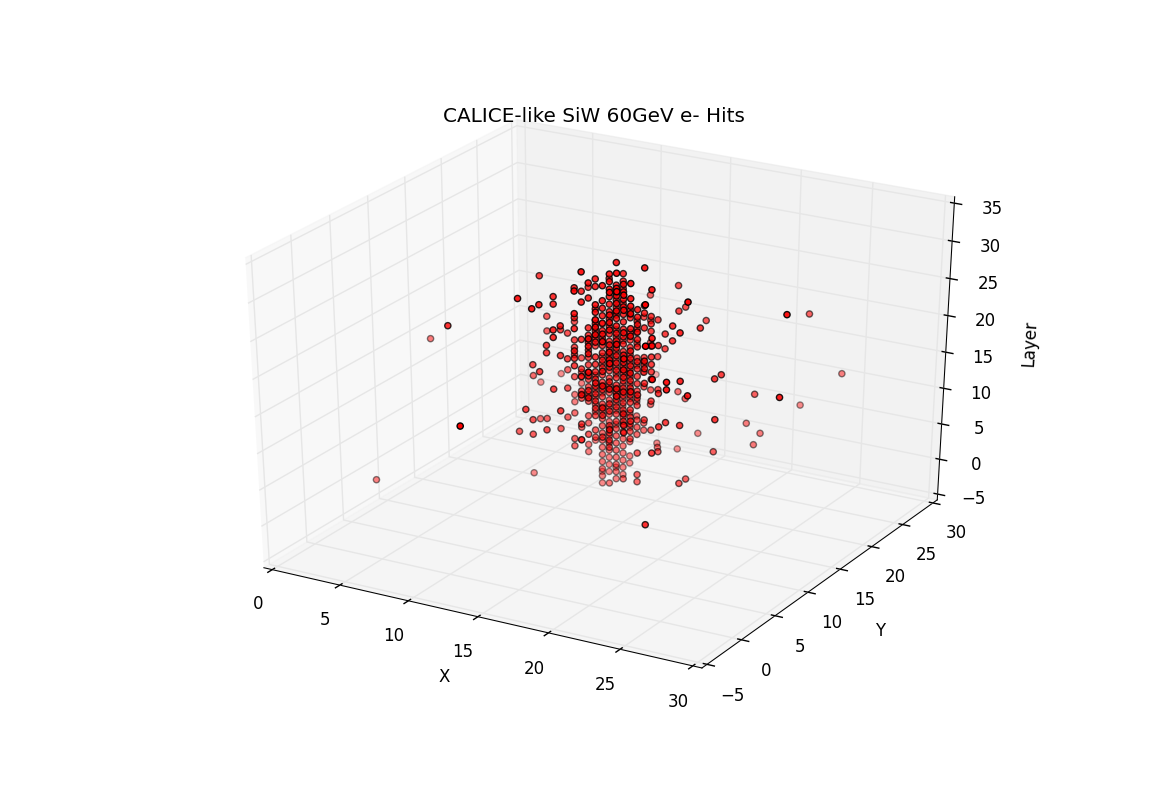
\includegraphics[width=0.9\textwidth]{figures/ch_simulations/hgc/scatter_3d/scatter_3D_60GeV.png}
    \caption{An example of a shower distribution within HGC for an incident 60 GeV $e^-$}
    \label{fig:simulations_hgc_scatter60}
 \end{figure}

\subsection{Analysis}
The objective of the readout analysis is to establish calorimeter performance characteristics: linearity of response and energy resolution. Not all systems are linear and intrinsically SiW-calorimeters are not linear in response. The reason for desirability of this characteristic is the ability to easily calibrate the device. In other words, given a linear system - the conversion of the raw response to energy is trivially established. In summary, the following steps are to be followed to etablish the performance characteristics:

\begin{itemize}
    \item Compute Total Response. In the case of SiW, we used right-hand side of equation~\ref{eq:simulations_hgc_totalResponse} to relate energy and total response.
    \item Overlay particle gun energy with total response as in Figure~\ref{fig:simulations_hgc_pblinearityresolution}. Perform a linear fit and extract the calibration coefficient.
    \item Using the derived calibration coefficient, compute the reconstructed energy distributions.
    \item Compute and overlay Resolution (according to equation~\ref{eq:simulations_hgc_resolution}) with incident energy. Perform the fit using equation~\ref{eq:simulations_hgc_resolutionfitfunc}.
\end{itemize}

\begin{center}
    \begin{equation}
        \label{eq:simulations_hgc_totalResponse}
         {E} = {CC} \times {Raw Response}. = {CC} \times {\sum_{i=1}^{n_{layers}} w_i \times  R_{i}}
    \end{equation}
\end{center}{}

\begin{center}
    \begin{equation}
        \label{eq:simulations_hgc_resolution}
         {Resolution} = {\frac{\mu_E}{\sigma_E}}
    \end{equation}
\end{center}

\begin{center}
    \begin{equation}
        \label{eq:simulations_hgc_resolutionfitfunc}
         {f(x)} = {\sqrt{\frac{\alpha^2}{x^2} + C^2}}
    \end{equation}
\end{center}

\subsection{Results}
Exercising the procedure described just above, we first obtain reconstructed energy distributions in figures~\ref{fig:simulations_hgc_pbenergyreco} and ~\ref{fig:simulations_hgc_wenergyreco}.

 \begin{figure}[hbp]
    \centering
    \includegraphics[width=0.95\textwidth]{figures/ch_simulations/hgc/performance/Pb/EnergyRECO.png}
    \caption{Reconstructed Energy Distributions with Lead Absorber.}
    \label{fig:simulations_hgc_pbenergyreco}
 \end{figure}

  \begin{figure}[hbp]
    \centering
    \includegraphics[width=0.95\textwidth]{figures/ch_simulations/hgc/performance/W/EnergyRECO.png}
    \caption{Reconstructed Energy Distributions with Tungsten Absorber.}
    \label{fig:simulations_hgc_wenergyreco}
 \end{figure}

A guassian fit is performed, resolution is computed and provided in figures~\ref{fig:simulations_hgc_pblinearityresolution} and ~\ref{fig:simulations_hgc_wlinearityresolution}.
 \begin{figure}[hbp]
    \centering
    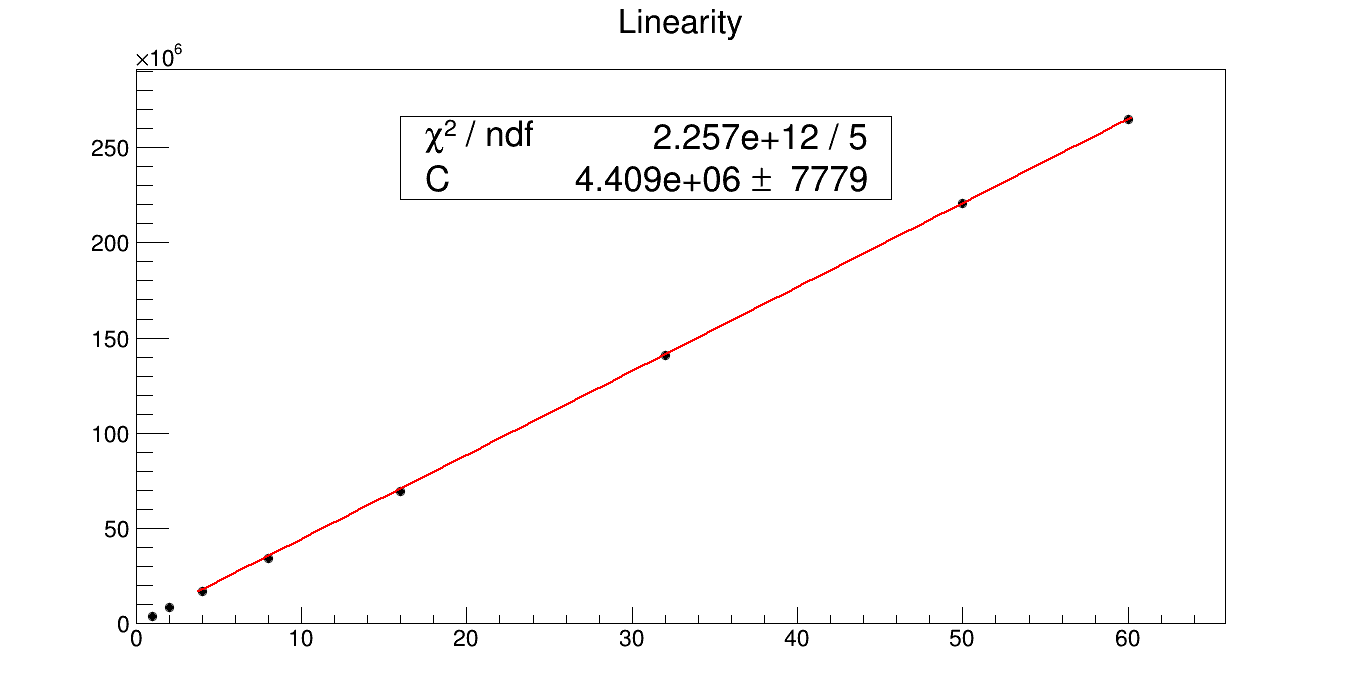
\includegraphics[width=0.9\textwidth]{figures/ch_simulations/hgc/performance/Pb/Linearity.png}
    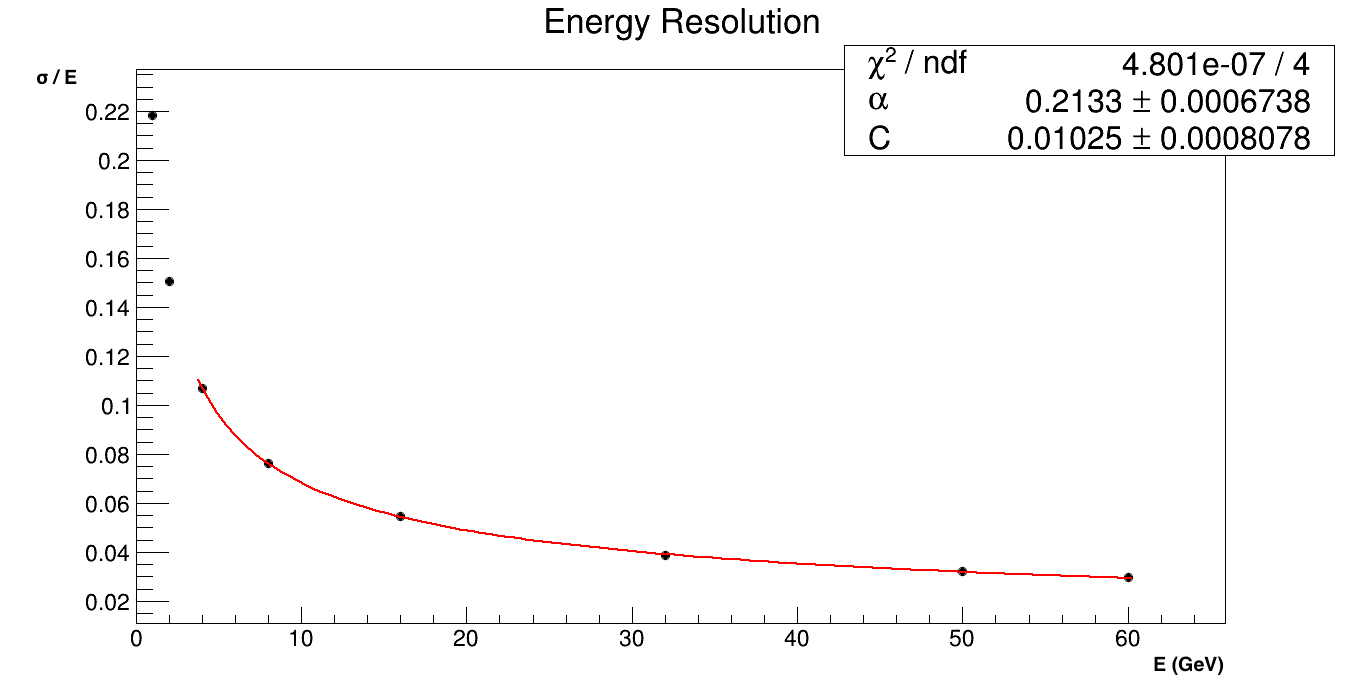
\includegraphics[width=0.9\textwidth]{figures/ch_simulations/hgc/performance/Pb/Resolution.png}
    \caption{Linearity (Top) and Energy Resolution (Bottom)}
    \label{fig:simulations_hgc_pblinearityresolution}
 \end{figure}

 \begin{figure}[hbp]
    \centering
    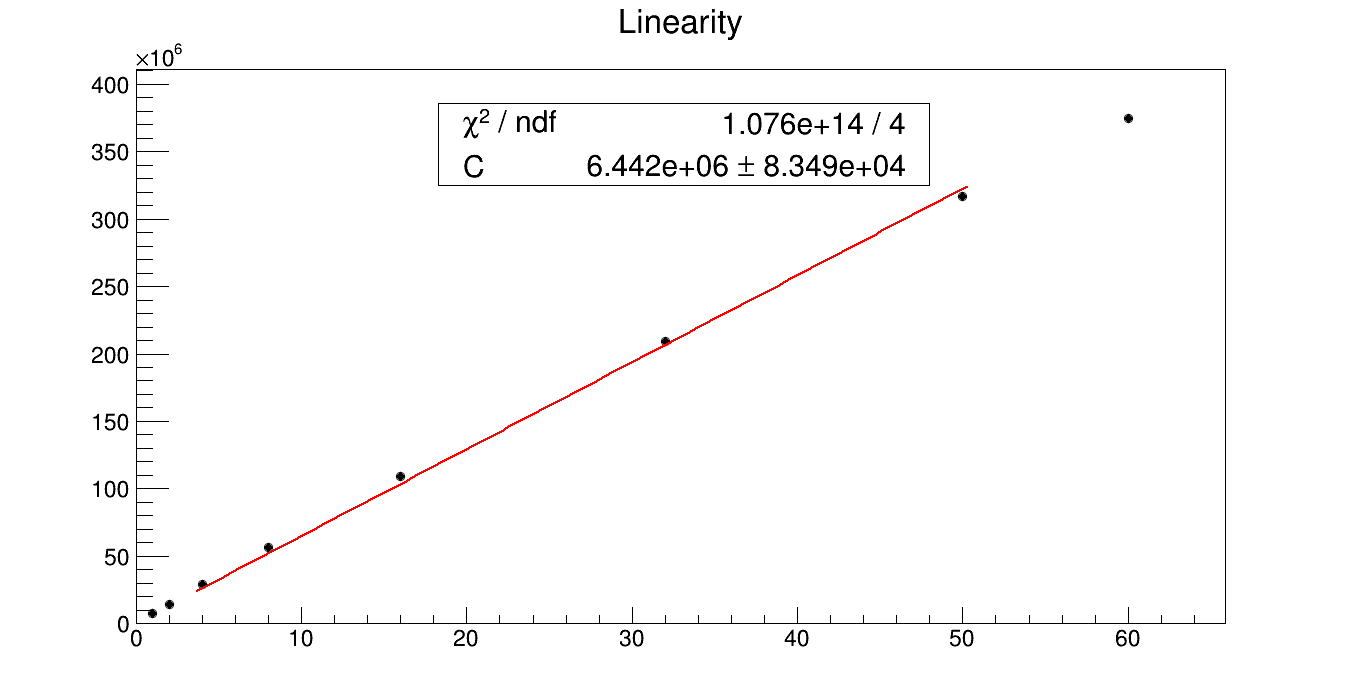
\includegraphics[width=0.9\textwidth]{figures/ch_simulations/hgc/performance/W/Linearity.png}
    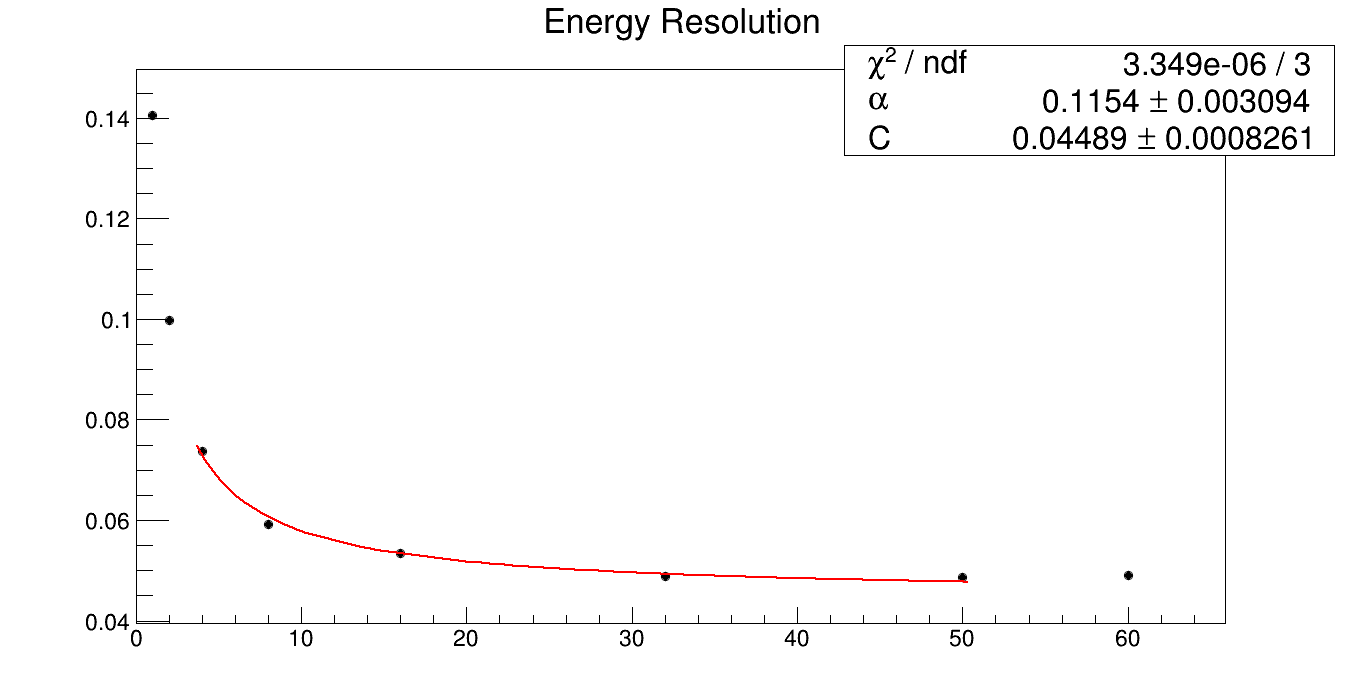
\includegraphics[width=0.9\textwidth]{figures/ch_simulations/hgc/performance/W/Resolution.png}
    \caption{Linearity (Top) and Energy Resolution (Bottom)}
    \label{fig:simulations_hgc_wlinearityresolution}
 \end{figure}